\chapter{As pessoas e a natureza}\label{ch:g5:people-and-nature}

Do alto de um morro, olhe o vale lá embaixo: campos em quadrados
caprichados, uma floresta manejada, margens de rio retificadas,
estradas, telhados. Quase nada do que está à vista cresceu assim
sozinho. Os seres humanos são a única \omterm{def:g5:biodiversity:species}{espécie} que remodela paisagens
inteiras conforme as necessidades dela --- e este capítulo olha com
honestidade para esse poder: o que ele nos dá, o que ele custa e
como pode ser bem usado.

\section{Paisagens feitas pelas pessoas}

\begin{proposition}[Quase toda paisagem é manejada]\label{prop:g5:people-and-nature:managed}
Quase toda paisagem ao nosso redor é moldada pelas pessoas:
\begin{itemize}
  \item as \emph{lavouras}\index{lavoura} são terrenos manejados em
        que uma \omterm{def:g1:plants-around-us:plant}{planta} escolhida --- trigo, milho, batata --- é
        cultivada no lugar da mistura selvagem;
  \item quase todas as \emph{florestas}\index{floresta (manejada)}
        são plantadas, desbastadas e colhidas como lavouras lentas;
  \item os \emph{campos} existem porque são ceifados ou pastados ---
        abandonados, viram capoeira e depois mata;
  \item cidades, estradas e represas redesenham a própria terra.
\end{itemize}
Os cantos ``intocados'' são a exceção, e quase todos são protegidos
de propósito.
\end{proposition}
\admitted

\begin{example}[Lendo o vale]\label{ex:g5:people-and-nature:valley}
Aquela vista do alto do morro, item por item: a lavoura de trigo
alimenta a padaria; as fileiras de pinheiros são uma lavoura de
madeira mais velha que o florestal que cuida dela; o campo florido é
ceifado todo mês de julho --- pule dois verões e as amoreiras
silvestres tomam conta; o rio foi retificado há muito tempo para
proteger as lavouras das cheias. O vale é uma oficina --- uma oficina
que funciona há séculos.
\end{example}

\begin{omfigure}
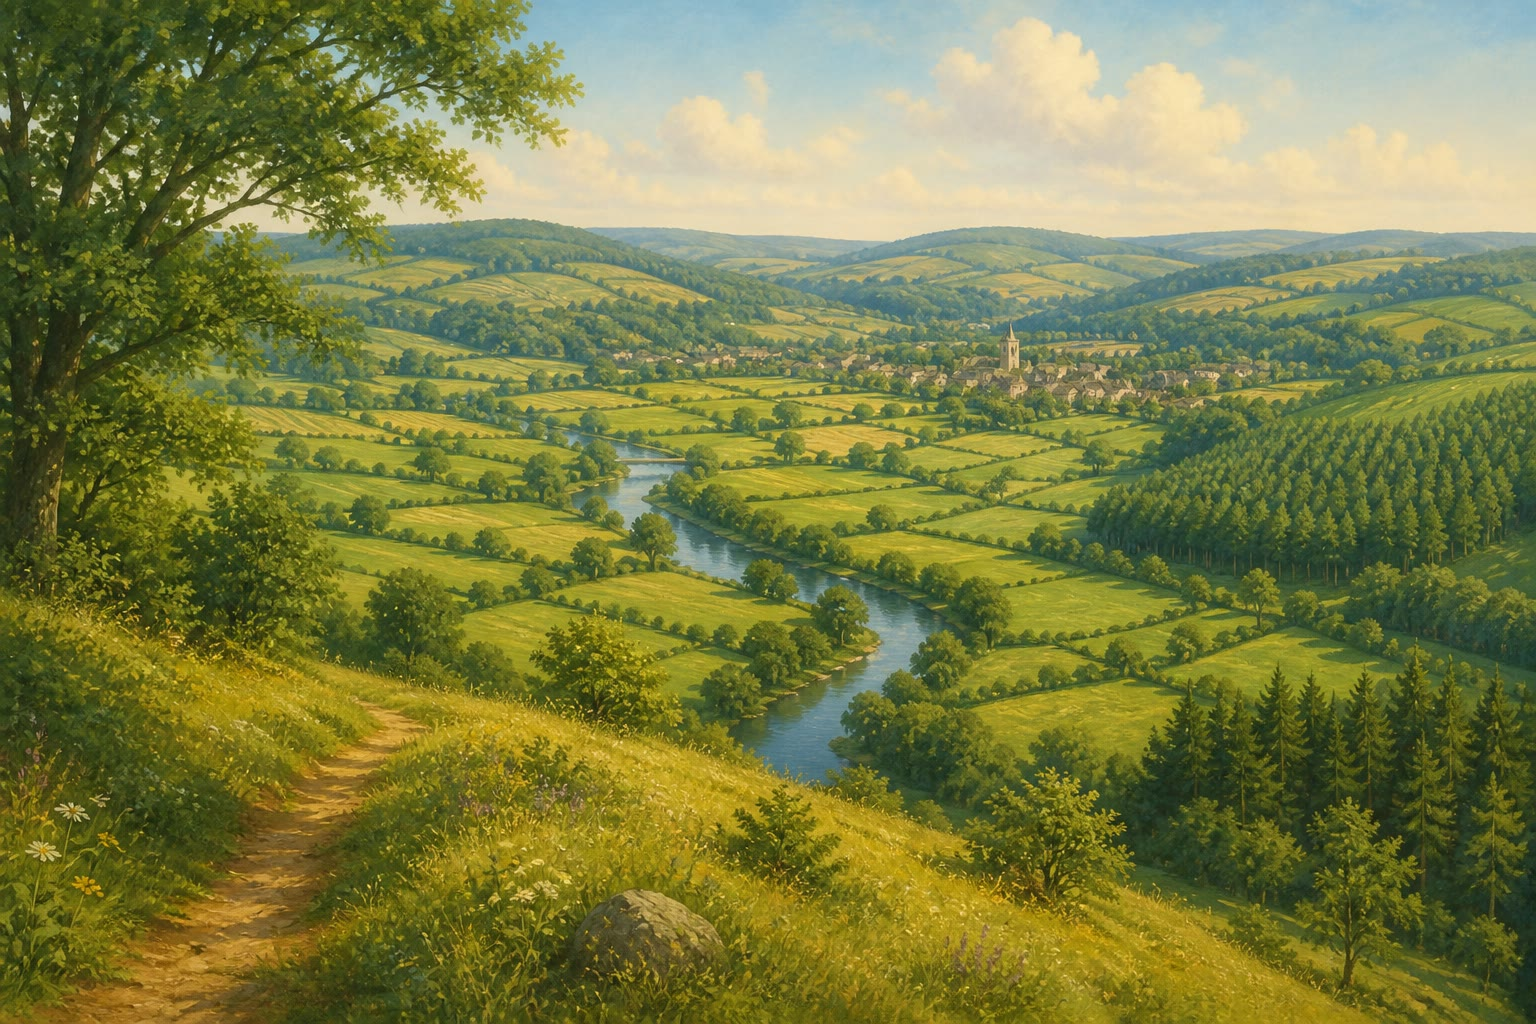
\includegraphics[width=0.62\linewidth]{images/book1/ai/g5-nature-valley.jpg}

{\small A vista do alto do morro: lavouras, cercas vivas, floresta
manejada, rio retificado, vilarejo --- uma paisagem de trabalho, com
séculos de idade.}
\end{omfigure}

\begin{remark}[Nem vilão nem enfeite de jardim]\label{rem:g5:people-and-nature:honest}
Seria falso contar esta história como pura destruição --- a
agricultura alimenta a humanidade, e uma zona rural com cercas vivas
pode ser rica em \omterm{def:g5:biodiversity:species}{espécies} (\cref{ex:g5:biodiversity:orchard}) --- e
igualmente falso fingir que remodelar não custa nada (a
\cref{prop:g5:biodiversity:loss} listou as contas). A pergunta
honesta nunca é ``mexer na natureza ou não?'', e sim ``como manejar
aquilo em que mexemos, de modo que continue funcionando --- para nós
e para o resto da teia?''.
\end{remark}

\section{Manejar bem e manejar mal}

\begin{example}[Dois jeitos de cultivar uma encosta]\label{ex:g5:people-and-nature:twofarms}
Encosta A: uma lavoura gigante, cercas vivas arrancadas, solo
descoberto o inverno inteiro. A chuva lava o solo solto morro abaixo;
os ajudantes do \cref{ex:g5:biodiversity:orchard} não têm casa; uma
única praga pode varrer a lavoura única sem encontrar oposição.
Encosta B: lavouras menores com as cercas vivas mantidas, solo
coberto durante o inverno, culturas alternadas ano a ano. As cercas
vivas seguram o solo e abrigam os comedores de pragas; o rodízio dá
descanso à terra. As duas encostas alimentam pessoas --- só uma delas
ainda vai alimentar daqui a cem anos.
\end{example}

\begin{proposition}[As regras do uso duradouro]\label{prop:g5:people-and-nature:lasting}
O uso da natureza dura quando respeita três regras:
\begin{enumerate}
  \item \emph{não tirar mais rápido do que ela repõe}: colher
        madeira no ritmo de crescimento da floresta, pescar no
        ritmo de reprodução do cardume --- a pesca em excesso da
        \cref{prop:g5:biodiversity:loss} é esta regra quebrada;
  \item \emph{guardar os trabalhadores}: a vida do solo, os
        polinizadores, os comedores de pragas --- os serviços
        gratuitos do \cref{exo:g5:biodiversity:11} --- precisam ter
        as casas deles preservadas;
  \item \emph{devolver o que se toma emprestado}: o ciclo do
        composto da \cref{rem:g4:what-plants-need:soil}, em todas as
        escalas.
\end{enumerate}
\end{proposition}
\admitted

\begin{example}[A aritmética do florestal]\label{ex:g5:people-and-nature:forester}
Uma floresta bem cuidada é a prova mais antiga de que a regra 1
funciona: quem cuida da floresta conta quanto ela cresce a cada ano e
não corta mais do que isso. A floresta então dá madeira todo ano,
para sempre --- e continua sendo floresta, com as corujas, os veados
e os besouros dela. Algumas \omterm{prop:g5:people-and-nature:managed}{florestas} manejadas pelo mundo vêm sendo
colhidas assim há muitas centenas de anos sem encolher.
\end{example}

\section{Cidades, e abrir espaço de novo}

\begin{example}[Natureza na cidade]\label{ex:g5:people-and-nature:city}
Uma cidade parece o oposto da natureza e, mesmo assim, também é um
\omterm{def:g2:where-animals-live:habitat}{hábitat} --- um \omterm{def:g2:where-animals-live:habitat}{hábitat} rochoso e estranho. Andorinhões fazem ninho em
``penhascos'' de concreto, raposas patrulham as lixeiras, \omterm{def:g1:plants-around-us:plant}{plantas}
silvestres rompem as juntas do asfalto. E quem mora na cidade pode
alargar as boas-vindas: parques, telhados verdes, \omterm{def:g3:flowers-fruits-seeds:parts}{flores} na varanda
para as abelhas, a lagoa de escola do
\cref{ex:g2:where-animals-live:schoolpond}. Os métodos do
\cref{met:g5:biodiversity:help} funcionam entre prédios também.
\end{example}

\begin{example}[Devolver as curvas a um rio]\label{ex:g5:people-and-nature:river}
O rio retificado do vale corria depressa e provocava cheias feias rio
abaixo; os \omterm{prop:g3:sorting-living-things:groups}{peixes} e as libélulas dele tinham ido embora junto com as
curvas. Hoje os engenheiros às vezes \emph{recurvam} rios assim: as
curvas restauradas e os campos alagados seguram a água, guardam as
cheias, e as cegonhas do \cref{ex:g5:biodiversity:storks} reencontram
os campos delas. O manejo pode funcionar na direção contrária ---
consertar também é manejar.
\end{example}

\begin{method}[Julgar um uso da natureza]\label{met:g5:people-and-nature:judge}
Diante de qualquer uso da terra ou da água --- uma fazenda, uma
pescaria, uma estrada planejada, um quintal:
\begin{enumerate}
  \item pergunte o que é \emph{retirado} e se isso é mais rápido do
        que a reposição (regra 1);
  \item pergunte que \emph{casas e trabalhadores} são mantidos ou
        perdidos (regra 2);
  \item pergunte o que é \emph{devolvido} --- e que resíduos ficam
        para trás (regra 3);
  \item depois julgue: isso poderia continuar por cem anos? Que
        única mudança melhoraria mais a resposta?
\end{enumerate}
\end{method}

\section{Exercícios}

\begin{exercise}[$\star$]\label{exo:g5:people-and-nature:1}
Dê quatro tipos de paisagem moldada por pessoas, tirados da
\cref{prop:g5:people-and-nature:managed}, cada um com aquilo para
que é manejado.
\end{exercise}

\begin{exercise}[$\star$]\label{exo:g5:people-and-nature:2}
O que acontece com um campo que deixa de ser ceifado ou pastado?
\end{exercise}

\begin{exercise}[$\star$]\label{exo:g5:people-and-nature:3}
Enuncie as três regras do uso duradouro.
\end{exercise}

\begin{exercise}[$\star$]\label{exo:g5:people-and-nature:4}
No \cref{ex:g5:people-and-nature:twofarms}, liste três diferenças
entre as duas encostas e o que cada diferença muda.
\end{exercise}

\begin{exercise}[$\star$]\label{exo:g5:people-and-nature:5}
Explique a aritmética do florestal. Que regra é essa, e o que a
floresta dá em troca --- por quanto tempo?
\end{exercise}

\begin{exercise}[$\star$]\label{exo:g5:people-and-nature:6}
Diga três moradores selvagens das cidades e que elemento da cidade
cada um usa como \omterm{def:g2:where-animals-live:habitat}{hábitat}.
\end{exercise}

\begin{exercise}[$\star$]\label{exo:g5:people-and-nature:7}
O que recurvar o rio restaurou --- para as pessoas e para a teia?
\end{exercise}

\begin{exercise}[$\star$]\label{exo:g5:people-and-nature:8}
Faça a experiência: escolha uma vista perto de casa --- rua, lavoura,
parque --- e liste tudo nela que as pessoas manejam, como no
\cref{ex:g5:people-and-nature:valley}. Sobrou alguma coisa sem
manejo?
\end{exercise}

\begin{exercise}[$\star\star$]\label{exo:g5:people-and-nature:9}
``Proteger a natureza quer dizer nunca mexer nela.'' Discuta usando o
campo ceifado da \cref{prop:g5:people-and-nature:managed} --- um
\omterm{def:g2:where-animals-live:habitat}{hábitat} que \emph{desaparece} sem o toque humano --- e a
\cref{rem:g5:people-and-nature:honest}.
\end{exercise}

\begin{exercise}[$\star\star$]\label{exo:g5:people-and-nature:10}
Rode o \cref{met:g5:people-and-nature:judge} na encosta A do
\cref{ex:g5:people-and-nature:twofarms}: que regras ela quebra, e que
única mudança a melhoraria mais?
\end{exercise}

\begin{exercise}[$\star\star\star$]\label{exo:g5:people-and-nature:11}
Uma frota pesqueira dobra a captura durante cinco anos esplêndidos;
no sexto, os cardumes sumiram e a frota fica parada. Explique os seis
anos com a regra 1 --- por que quebrar essa regra \emph{parecia}
sucesso no começo? Compare com a aritmética oposta do florestal.
\end{exercise}
